\begin{frame}{Mediciones con el perfilador}

    \begin{onlyenv}<1>
        Calibración del instrumento, medición del colimador F280FC del SPIM
        \begin{columns}[t]
            \begin{column}{0.5\textwidth}
                \begin{figure}[H]
                \centering
                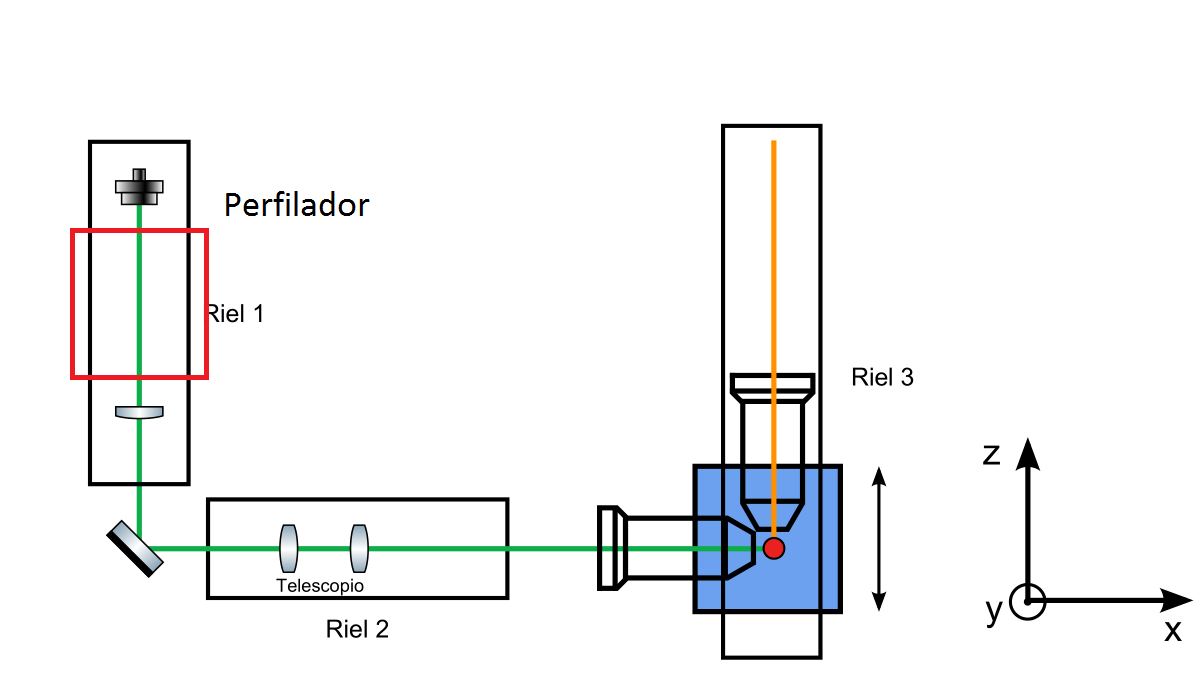
\includegraphics[width=\textwidth]{fig/perfilador/spim_riel_perfilador.png}
                \label{fig:spim_riel_perfilador}
                \end{figure}
                
                 \begin{itemize}
                    \item Inicio del riel:\\ $\sigma = (3,03 \pm 0,15)\,\text{mm}$
                \end{itemize}
                
            \end{column}

            \begin{column}{0.5\textwidth}
                \vspace{-2em}
                \begin{figure}[H]
                    \centering
                    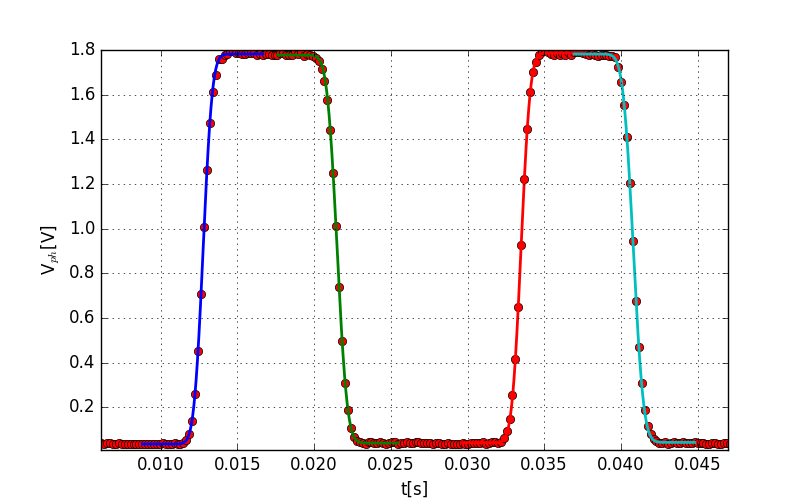
\includegraphics[width=\textwidth]{fig/perfilador/spim_foco_zoom.png}
                    \label{fig:spim_foco_zoom}
                \end{figure}
                \vspace{1em}
                \begin{itemize}
                    \item Fin del riel:\\ $\sigma = (3,02 \pm 0,18)\,\text{mm}$
                \end{itemize}
                
            \end{column}
            
        \end{columns}
        
       
    \end{onlyenv}
    
    \begin{onlyenv}<2>
        Medición manual del colimador F280FC del SPIM
            \begin{figure}[H]
                \centering
                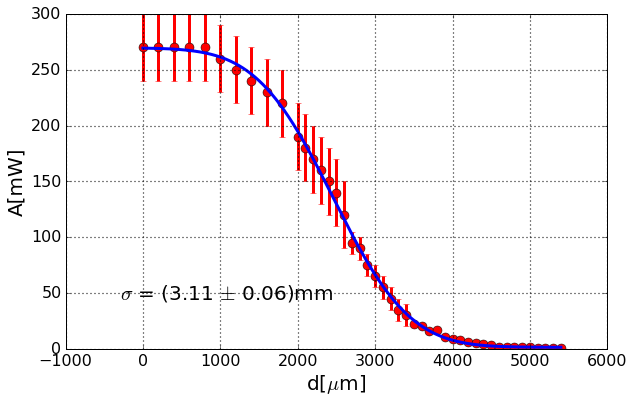
\includegraphics[width=0.7\textwidth]{fig/perfilador/calibracion_f280.png}
                \label{fig:perfilador/calibracion_f280}
            \end{figure}

        
    \end{onlyenv}


    \begin{onlyenv}<3>

        Haz en el telescopio del SPIM
        \begin{columns}[c]
        \begin{column}{0.5\textwidth}
            \begin{figure}[H]
                \centering
                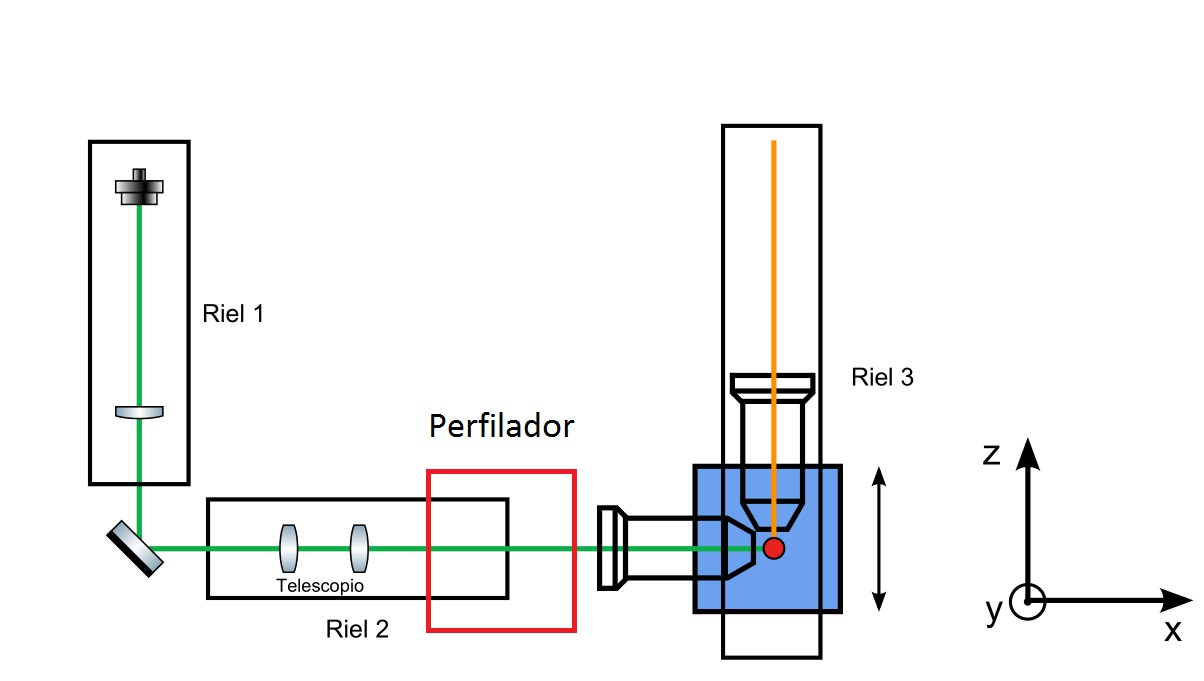
\includegraphics[width=\textwidth]{fig/perfilador/spim_lightsheet_perfilador}
                \label{fig:spim_lightsheet_perfilador}
            \end{figure}
        \end{column}
        \begin{column}{0.5\textwidth}
            \vspace{-3em}
            \begin{figure}[H]
                \centering
                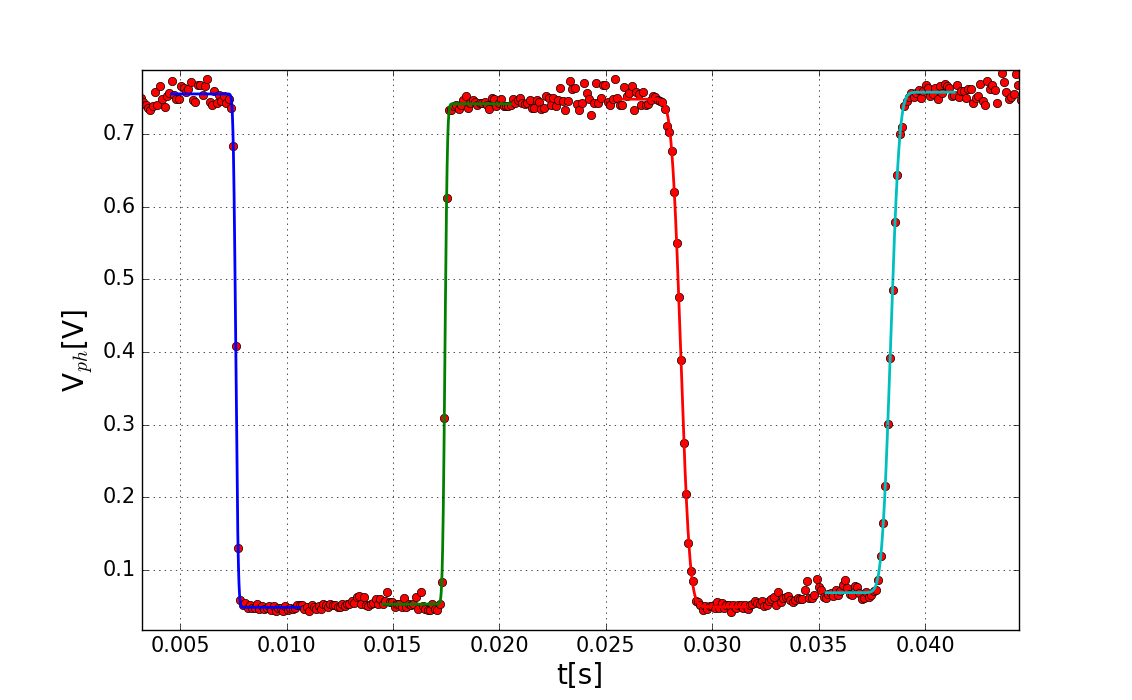
\includegraphics[width=\textwidth]{fig/perfilador/spim_lightsheet}
                \label{fig:spim_lightsheet}
            \end{figure}
            \vspace{-1em}
            Medición a \\d$\approx$80$\,$mm del fin del telescopio
            $\sigma_1 = (0,55 \pm 0,02)\,\text{mm}$\\
            $\sigma_2 = (2,11 \pm 0,05)\,\text{mm}$\\
            \end{column}
        \end{columns}
        \vspace{1em}
        %Las transiciones acusan una \underline{divergencia} apreciable, como es de esperar en un telescopio.
    \end{onlyenv}
\end{frame}


\begin{frame}{Mediciones con el polarimetro}
    \begin{onlyenv}<1>
        Calibración de láminas polarizadoras
        \begin{columns}
            \begin{column}{0.5\textwidth}
                \begin{figure}[H]
                \centering
                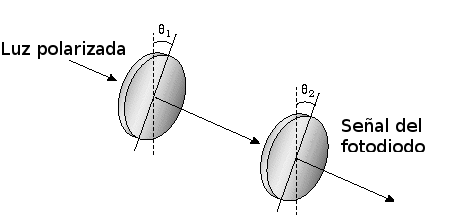
\includegraphics[width=\textwidth]{fig/polarimetro/calibracion}
                \label{fig:polarimetro_calibracion}
            \end{figure}
            \end{column}
            \begin{column}{0.5\textwidth}
                \begin{itemize}
                    \item Con dos polarizadores móviles se puede terminar los parámetros del material polarizador
                    \item El plástico usado tiene la siguiente matriz de transmisión $\begin{pmatrix} 0,5 & 0 \\ 0 & 2\times 10^{-6} \end{pmatrix}$
                    \item Permite polarizar, pero elimina un \%50 de la señal en el máximo.
                \end{itemize}
            \end{column}
        \end{columns}
    \end{onlyenv}
    \begin{onlyenv}<2>
        Medición de polarización par láser azul DHOM-M-473  
        \begin{columns}
            \begin{column}{0.5\textwidth}
                Antes de la fibra óptica
                \begin{figure}[H]
                    \centering
                    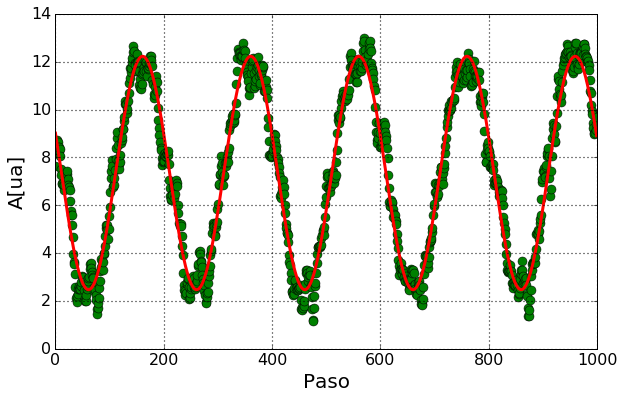
\includegraphics[width=\textwidth]{fig/polarimetro/polarizacion_azul}
                    \label{fig:polarimetro_calibracion}
                \end{figure}
                $\frac{\max - \min}{\max + \min} = (0.83 \pm 0.39)$
            \end{column}
            \begin{column}{0.5\textwidth}
            
                Después de la fibra óptica
                \begin{figure}[H]
                    \centering
                    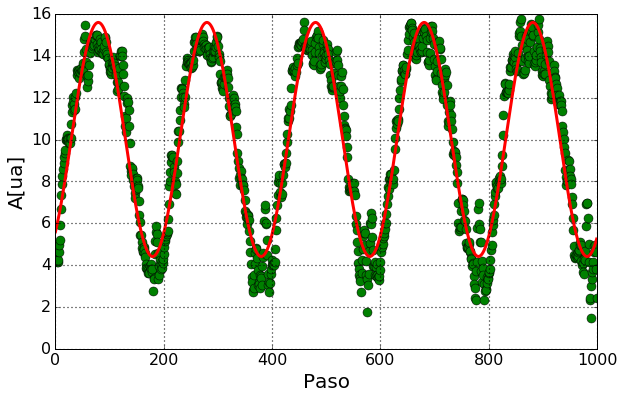
\includegraphics[width=\textwidth]{fig/polarimetro/polarizacion_azul_fibra}
                    \label{fig:polarimetro_calibracion}
                \end{figure}
                $\frac{\max - \min}{\max + \min} = (0.83 \pm 0.31)$
            \end{column}
        \end{columns}
    \end{onlyenv}
\end{frame}
